\documentclass[10pt,ngerman]{beamer}

% https://ctan.org/pkg/fontenc
\usepackage[T1]{fontenc}

% https://www.ctan.org/pkg/lm
\usepackage{lmodern}

% https://www.ctan.org/pkg/inputenc
\usepackage[utf8]{inputenc}

% https://ctan.org/pkg/graphicx
\usepackage{graphicx}
\graphicspath{ {./images/} }

% https://ctan.org/pkg/babel
\usepackage{babel}

% https://ctan.org/pkg/amsmath
\usepackage{amsmath}

% https://ctan.org/pkg/siunitx
\usepackage{siunitx}
\sisetup{locale=DE}

% https://ctan.org/pkg/url
\usepackage{url}

% https://ctan.org/pkg/microtype
\usepackage{microtype}

% https://ctan.org/pkg/float
\usepackage{float}

% https://ctan.org/pkg/multicol
\usepackage{multicol}

% https://ctan.org/pkg/blindtext
\usepackage{blindtext}

\usepackage{tikz}
\usepackage{mathtools}

% from https://stackoverflow.com/a/44662211/20453714
\usepackage{chngcntr}
\counterwithin{figure}{section}

% from https://tex.stackexchange.com/a/127150
\setbeamertemplate{caption}[numbered]

\title{TI-Nspire CAS}
\author{Erik Graumann}
\institute[TSS]{Theodor-Storm-Schule Husum}
\date{2024-06-11}

\begin{document}

\frame{\titlepage}

\begin{frame}
	\frametitle{Inhaltsverzeichnis}
	\tableofcontents
\end{frame}

\section{Beschränkung}

\begin{frame}
	\frametitle{Beschränkung}

	Mit dem Symbol | kann man einem Ausgedruck Beschränkungen geben. \newline

	\textbf{Beispiel}

	\begin{equation}
		\operatorname{solve}(\sin \alpha = 2 \cdot \cos x) \xRightarrow{TI} x = \textbf{n1} \cdot \pi-\tan^{-1}\left(\frac{1}{2}\right) + \frac{\pi}{2}
	\end{equation}
	\begin{equation}
		\operatorname{solve}(\sin \alpha = 2 \cdot \cos x)\ \vert \ 0 \le \alpha\ \text{and}\ \alpha \le \pi \xRightarrow{TI} x = \frac{\pi}{2} - \tan^{-1}\left(\frac{1}{2}\right)
	\end{equation}

\end{frame}

\subsection{Beschränkung auf Zahlenräume}

\begin{frame}
	\frametitle{Zahlenräume}

	Mit \(\text{\textbf{\textit{n1}}}\) oder \(\text{\textbf{\textit{c1}}}\) kann man innerhalb einer Beschränkung, Variablen auf einen Zahlenraum festlegen.

\end{frame}

\section{Approximierung in Brüche}

\begin{frame}
	\frametitle{Approximierung in einen Bruch}

	Mit \(\blacktriangleright\operatorname{approxFraction}()\) kann man beliebige Werte zu einem Brauch annähern. Der Funktionswert bestimmt die Genauigkeit. Zu finden ist es unter "Werkzeuge - Zahl - In Bruch approximieren" \newline

	\textbf{Beispiel}

	\begin{equation}
		0.333333 \blacktriangleright\operatorname{approxFraction}(1 \cdot 10^{-6}) \xRightarrow{TI} \frac{1}{3}
	\end{equation}


\end{frame}

\section{Kleine Hilfsfunktionen}

\begin{frame}
	\frametitle{Kleine Hilfen}

	\textbf{\textit{zeros}}\((Ausdruck, Variable)\) gibt fast das selbe Ergebnis, wie \textbf{\textit{solve}}\((\operatorname{f}(x)=0, x)\) wieder, jedoch werden nur exakte Lösungen wiedergegeben. \newline

	\textbf{\textit{tangentLine}}(Ausdruck, Variable, Punkt) gibt einem die Tangente an einem beliebigen Punkt einer Funktion. \newline

	\textbf{\textit{unitV}}(Vektor) gibt den Einheitsvektor eines gegebenen Vektors wieder.

\end{frame}

\section{3D-Darstellung im TI}

\subsection{Aufrufen der 3D-Darstellung}

\begin{frame}
	\frametitle{Aufrufen der 3D-Darstellung}

	\begin{columns}
		\begin{column}{0.5\textwidth}
			Zu finden ist die 3D-Darstellung unter ''Werkzeuge - 3D-Darstellung'' innerhalb einer Graph-Seite.
		\end{column}

		\begin{column}{0.5\textwidth}
			\begin{figure}
				\centering
				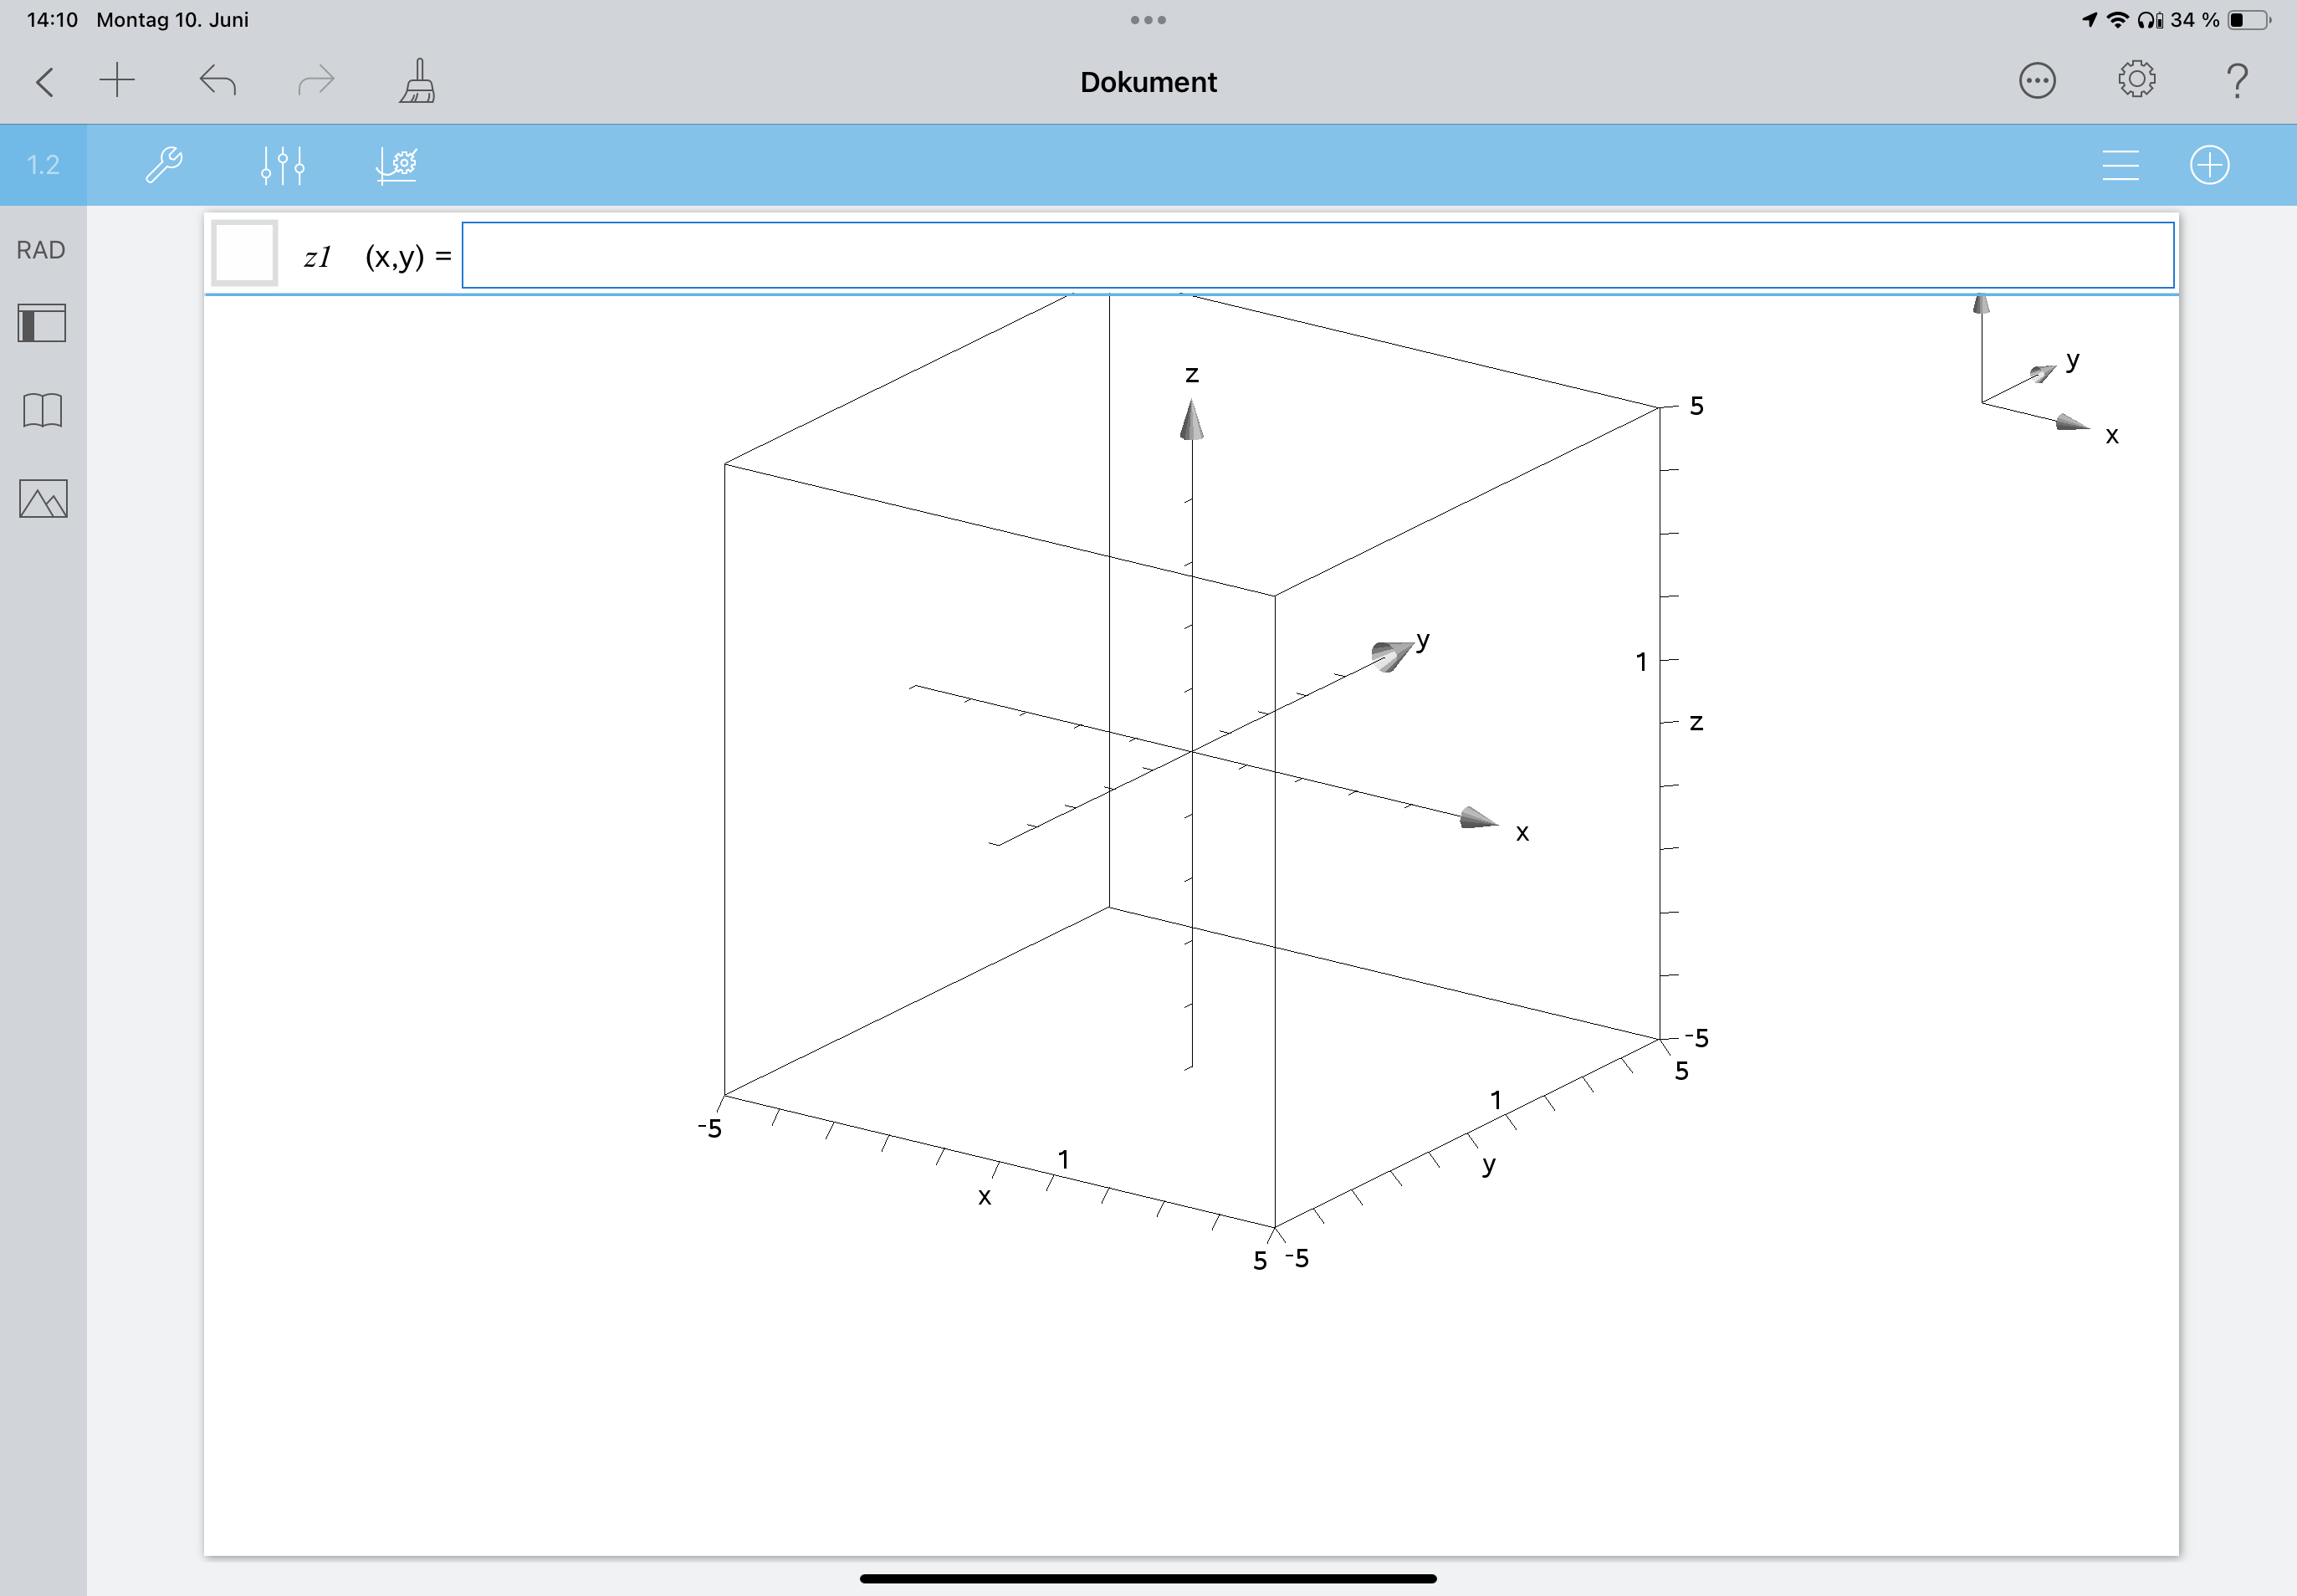
\includegraphics[width=\textwidth]{IMG_1444.png}
				\caption{3D-Darstellung}
			\end{figure}
		\end{column}
	\end{columns}

\end{frame}

\subsection{Arten der 3D-Darstellung}

\begin{frame}
	\frametitle{Arten der 3D-Darstellung}

	\begin{columns}
		\begin{column}{0.5\textwidth}
			\begin{figure}
				\centering
				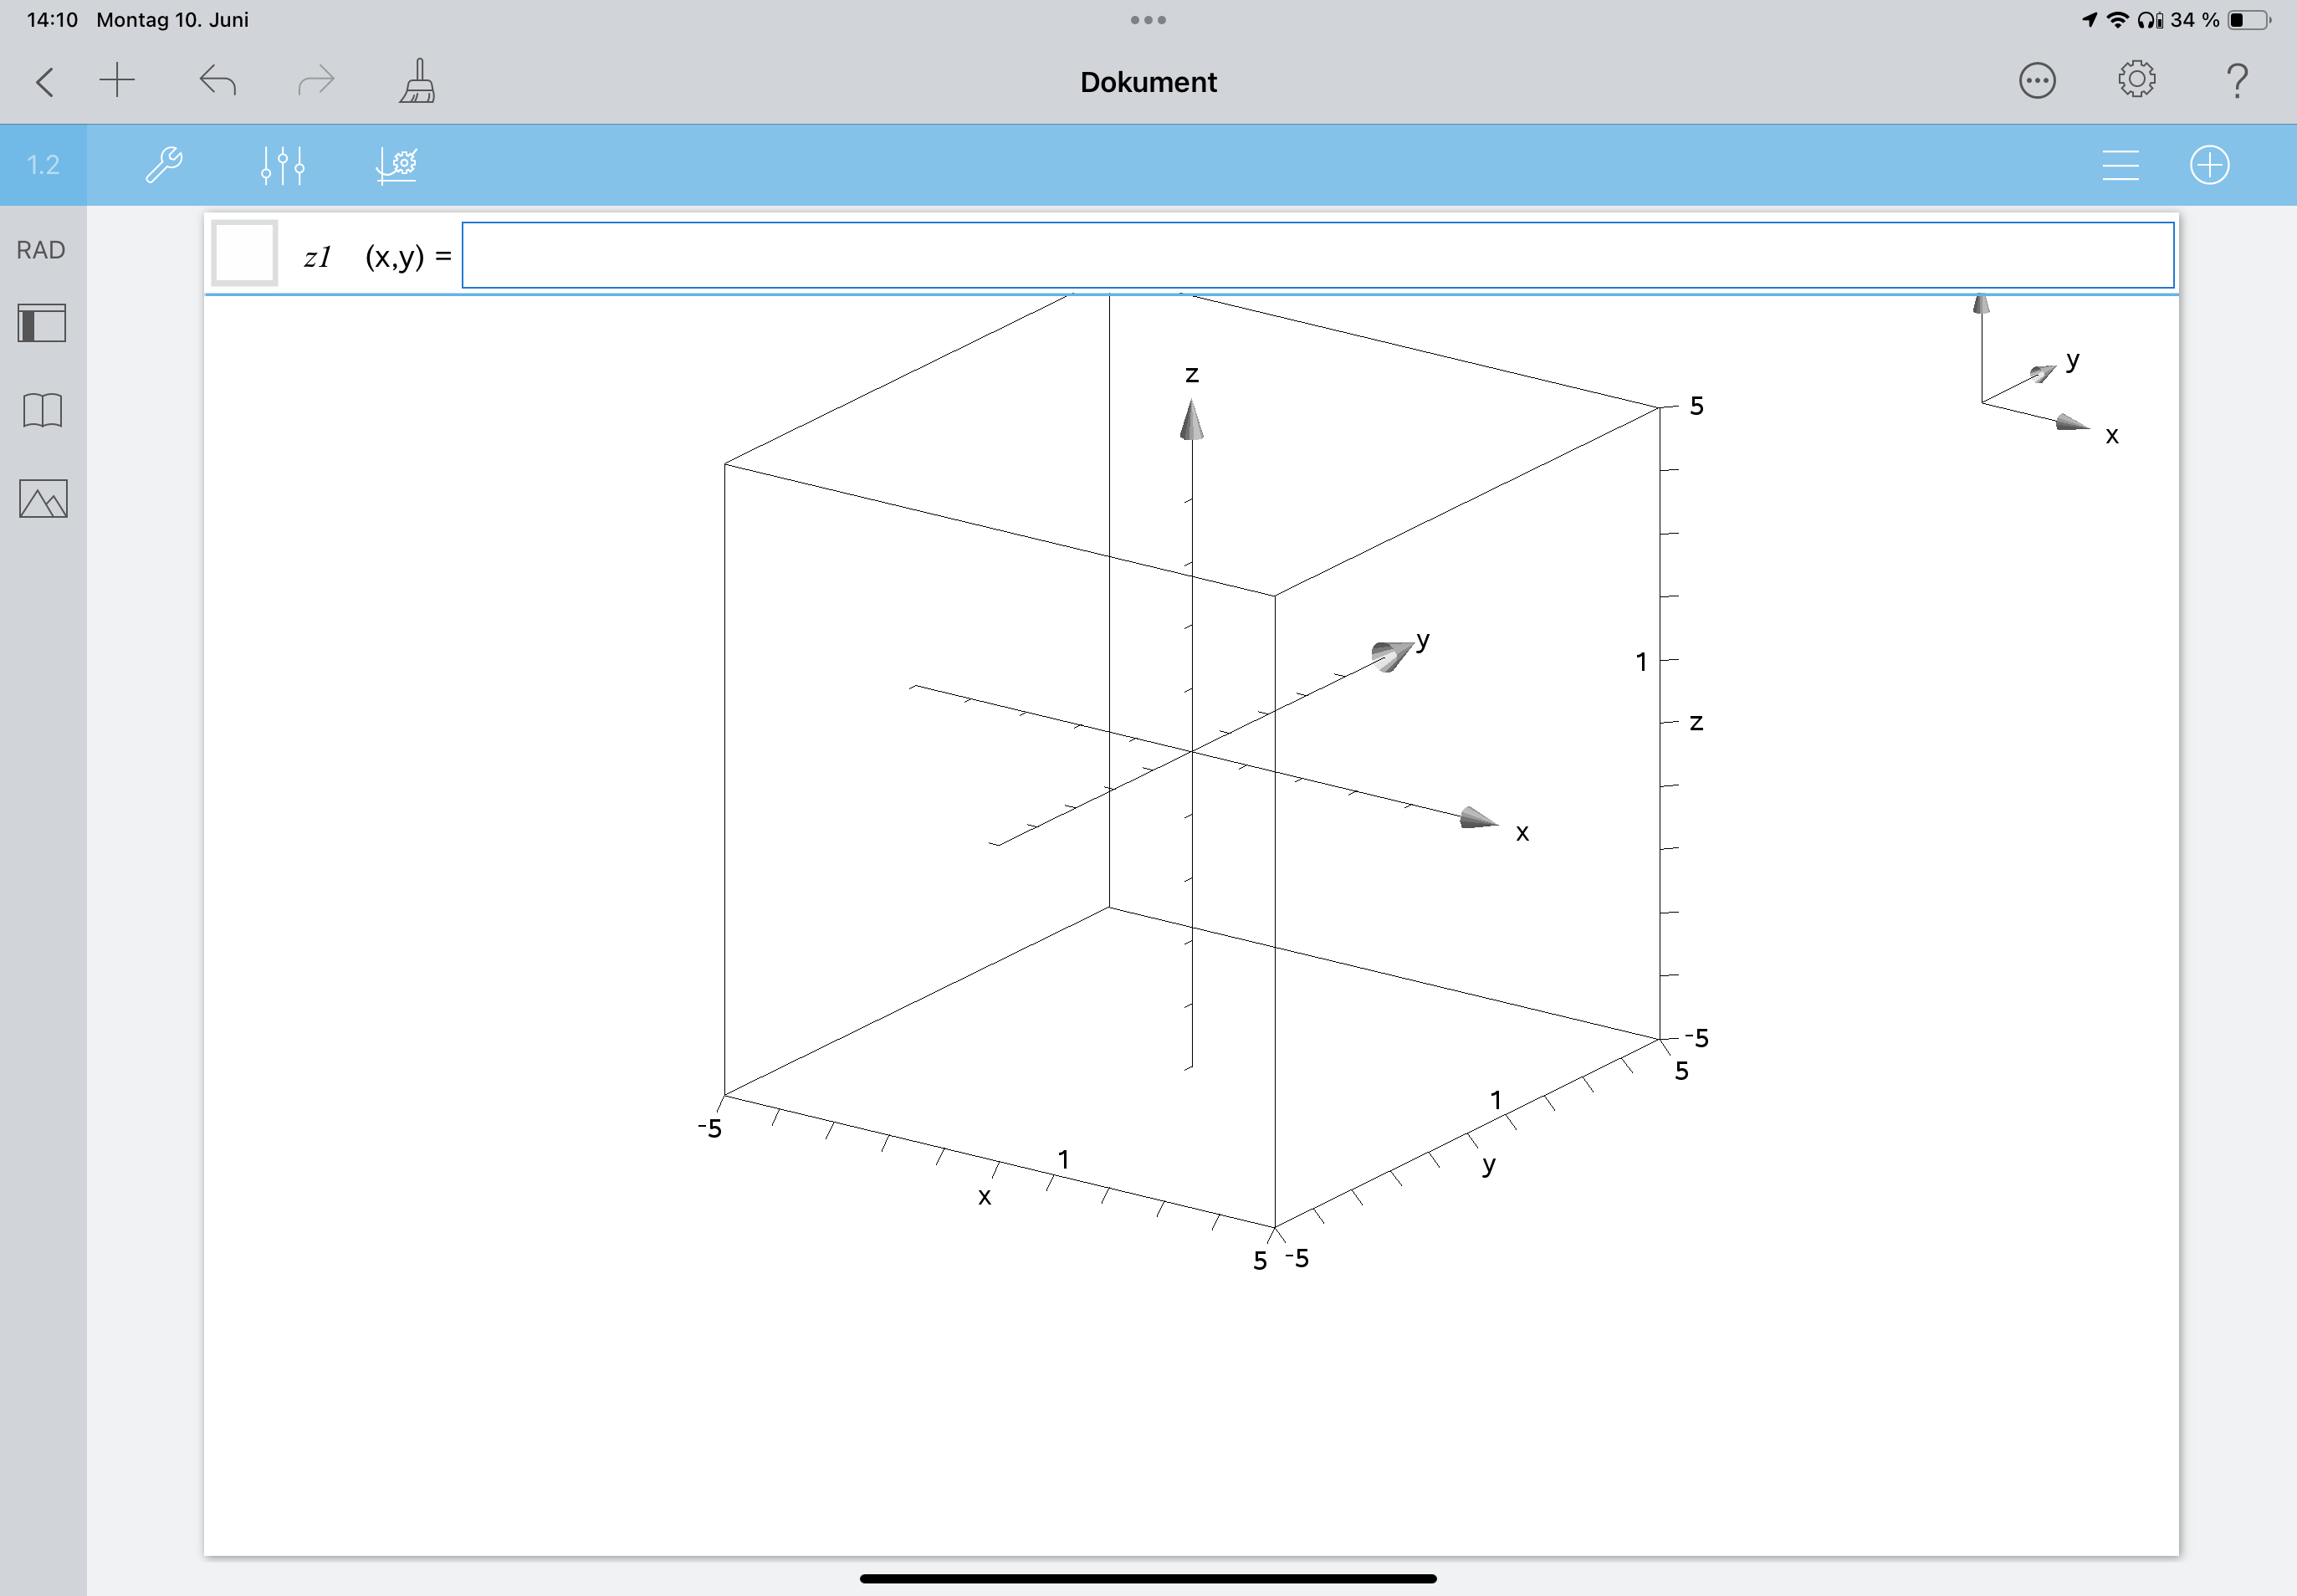
\includegraphics[width=\textwidth]{IMG_1444.png}
				\caption{3D-Darstellung im Funktions-Modus}
				\label{fig:Funktions-Modus}
			\end{figure}
		\end{column}

		\begin{column}{0.5\textwidth}
			\begin{figure}
				\centering
				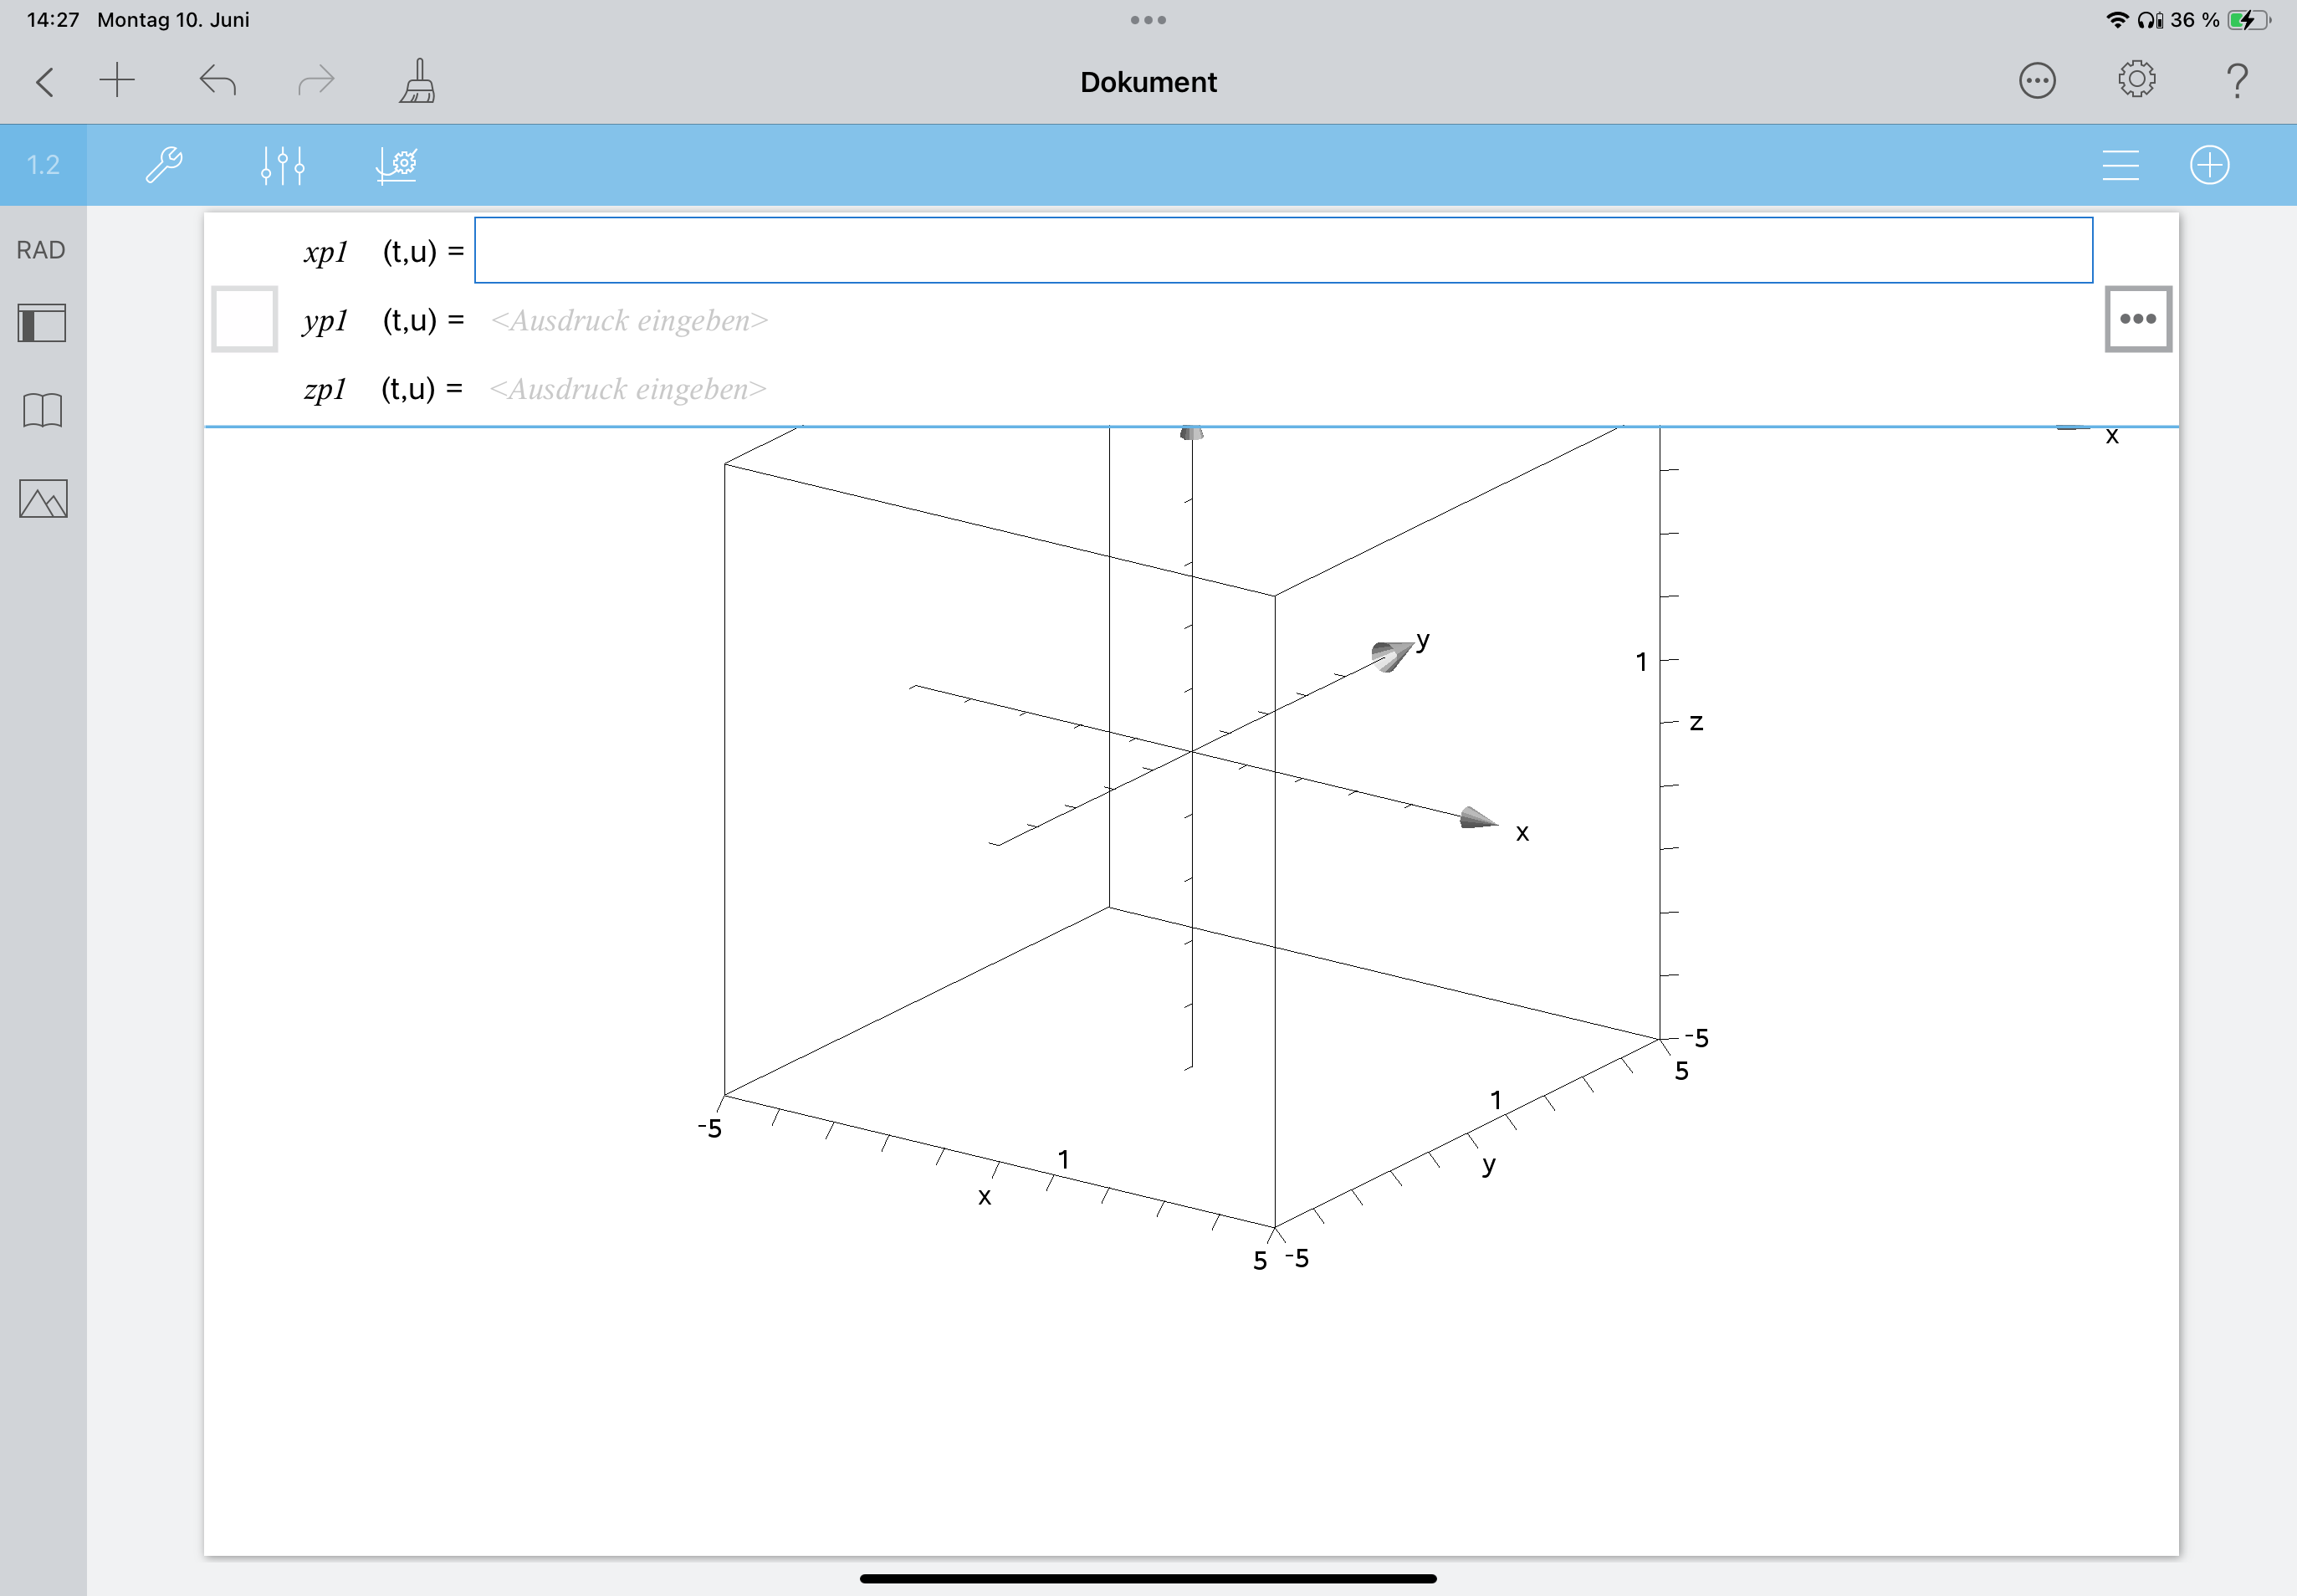
\includegraphics[width=\textwidth]{IMG_1445.png}
				\caption{3D-Darstellung im Parameter-Modus}
				\label{fig:Parameter-Modus}
			\end{figure}
		\end{column}
	\end{columns}
\end{frame}

\subsection{Darstellung von Ebenen}

\begin{frame}
	\frametitle{Ebenen}

	\begin{columns}
		\begin{column}{0.5\textwidth}
			\begin{figure}
				\centering
				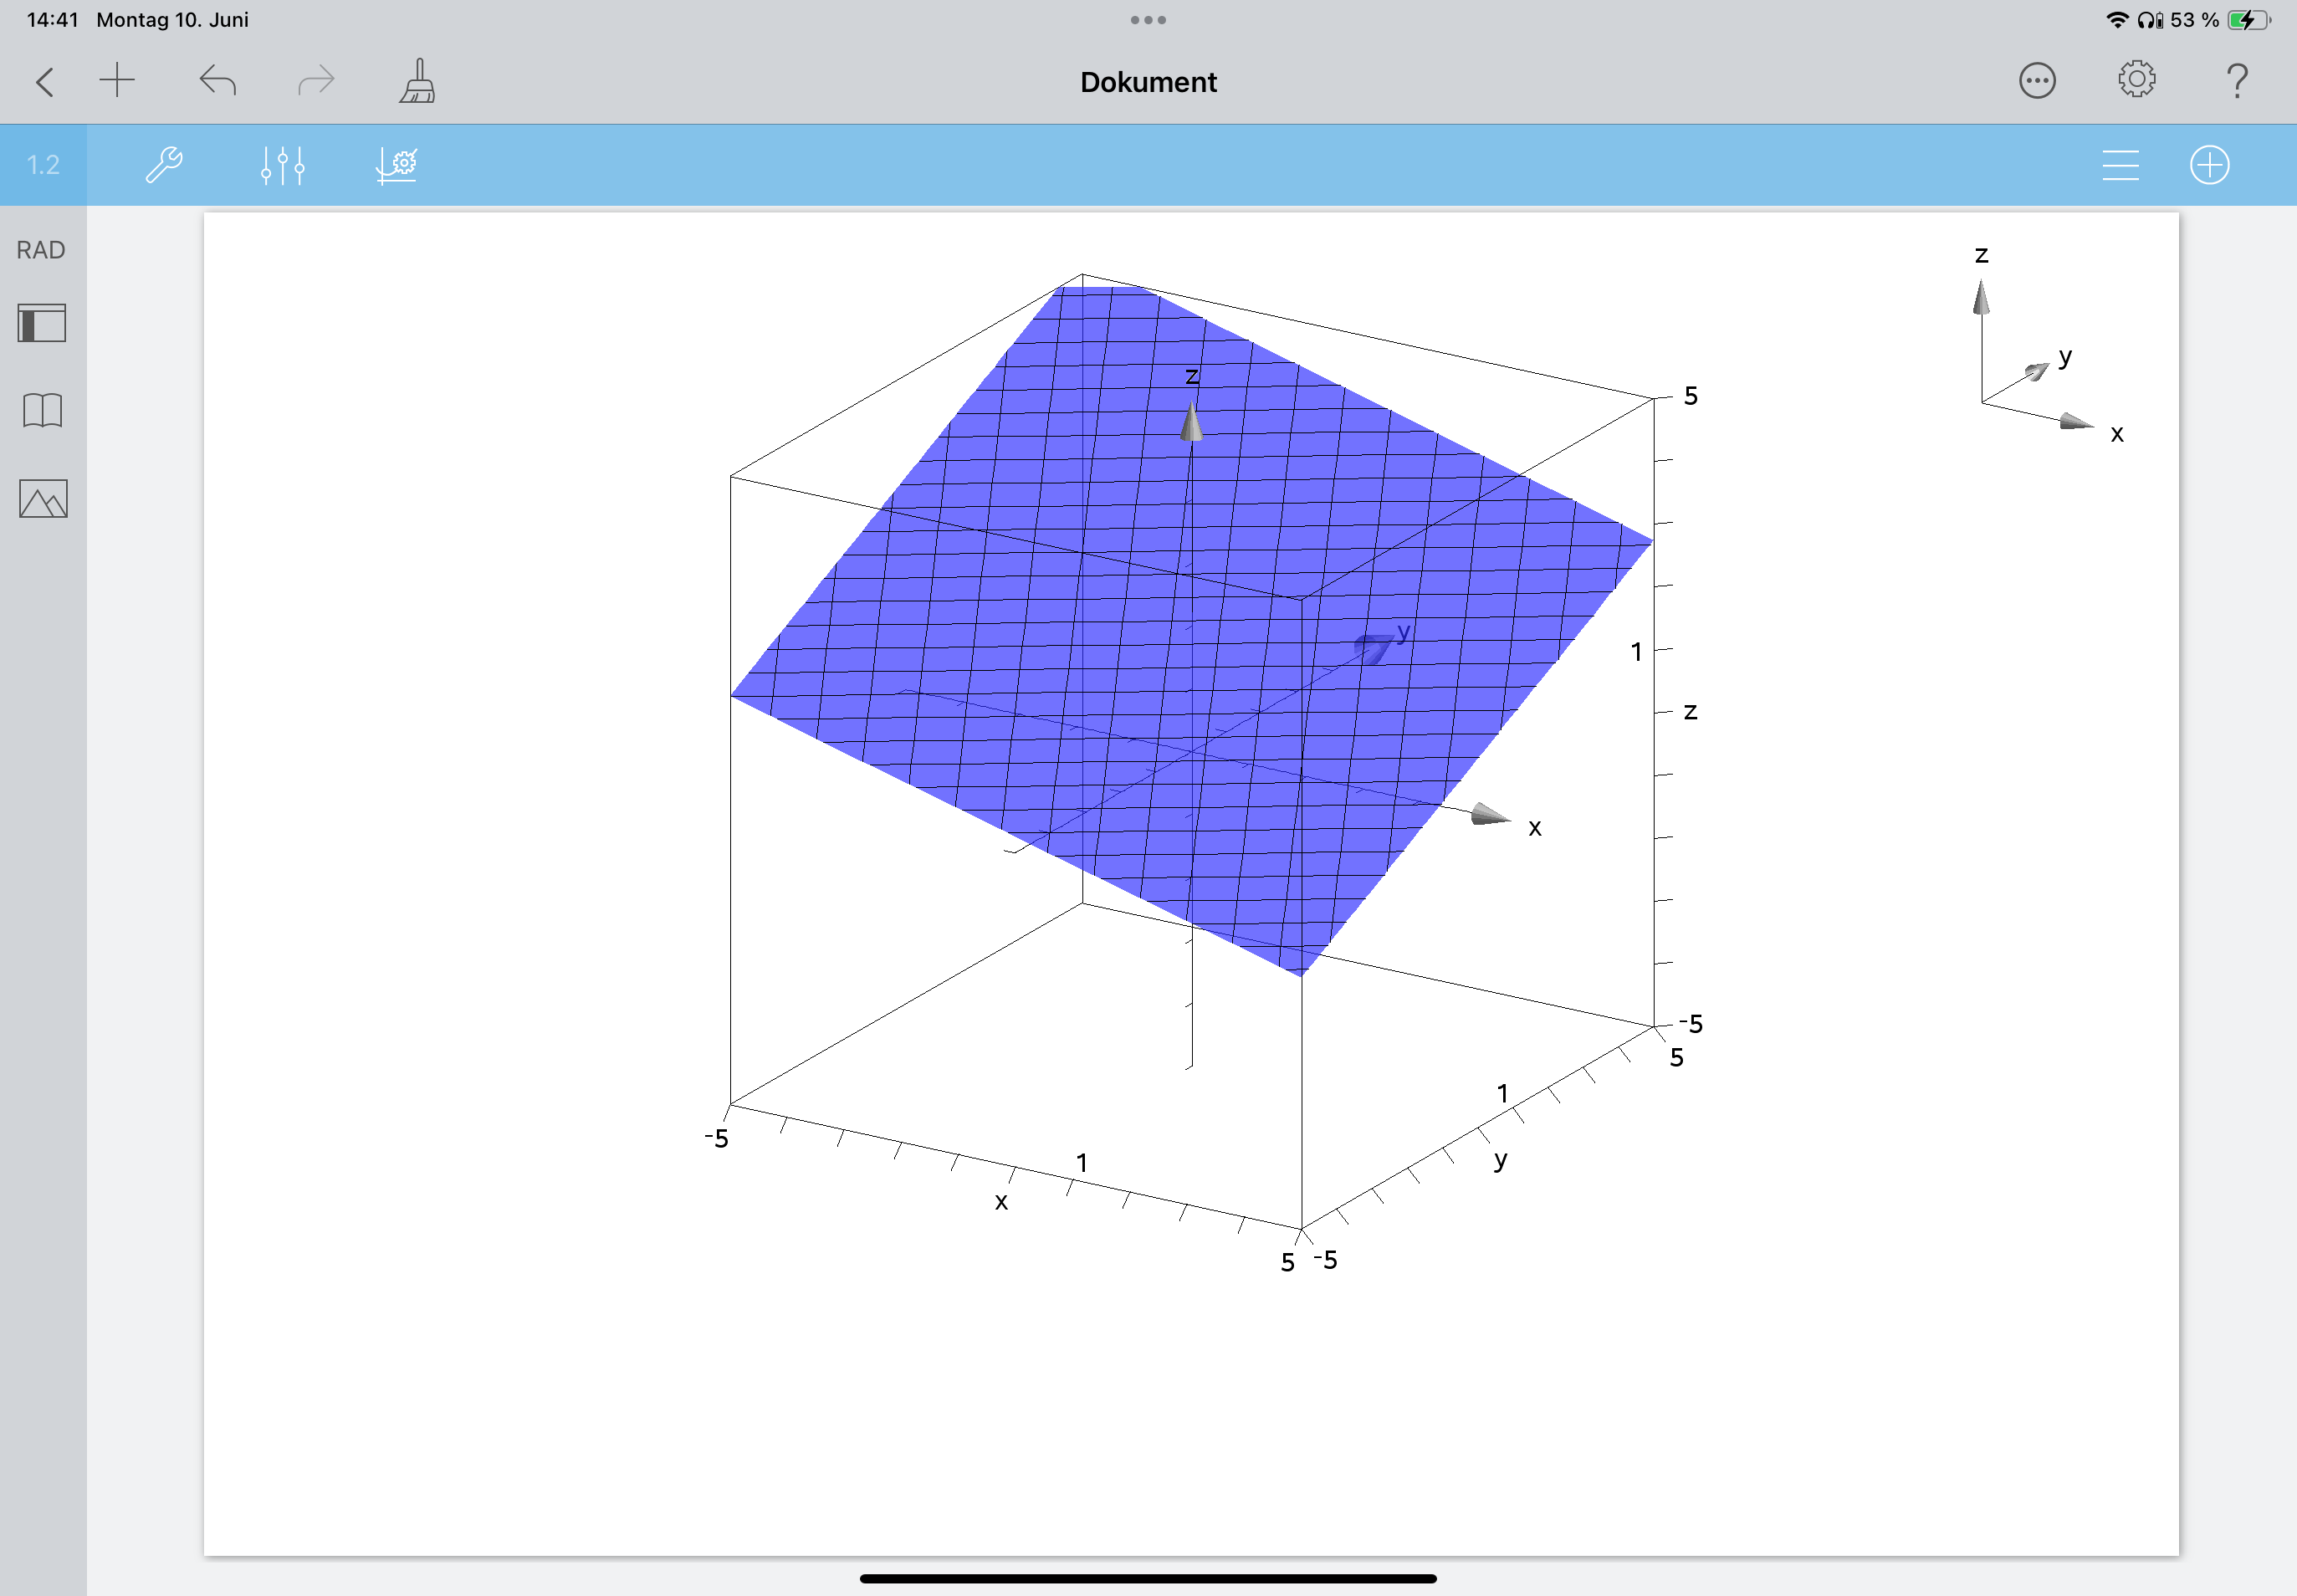
\includegraphics[width=\textwidth]{IMG_1446.png}
				\caption{Darstellung von einer Ebene}
				\label{fig:Darstellung-Ebene}
			\end{figure}
		\end{column}

		\begin{column}{0.5\textwidth}
			\begin{figure}
				\centering
				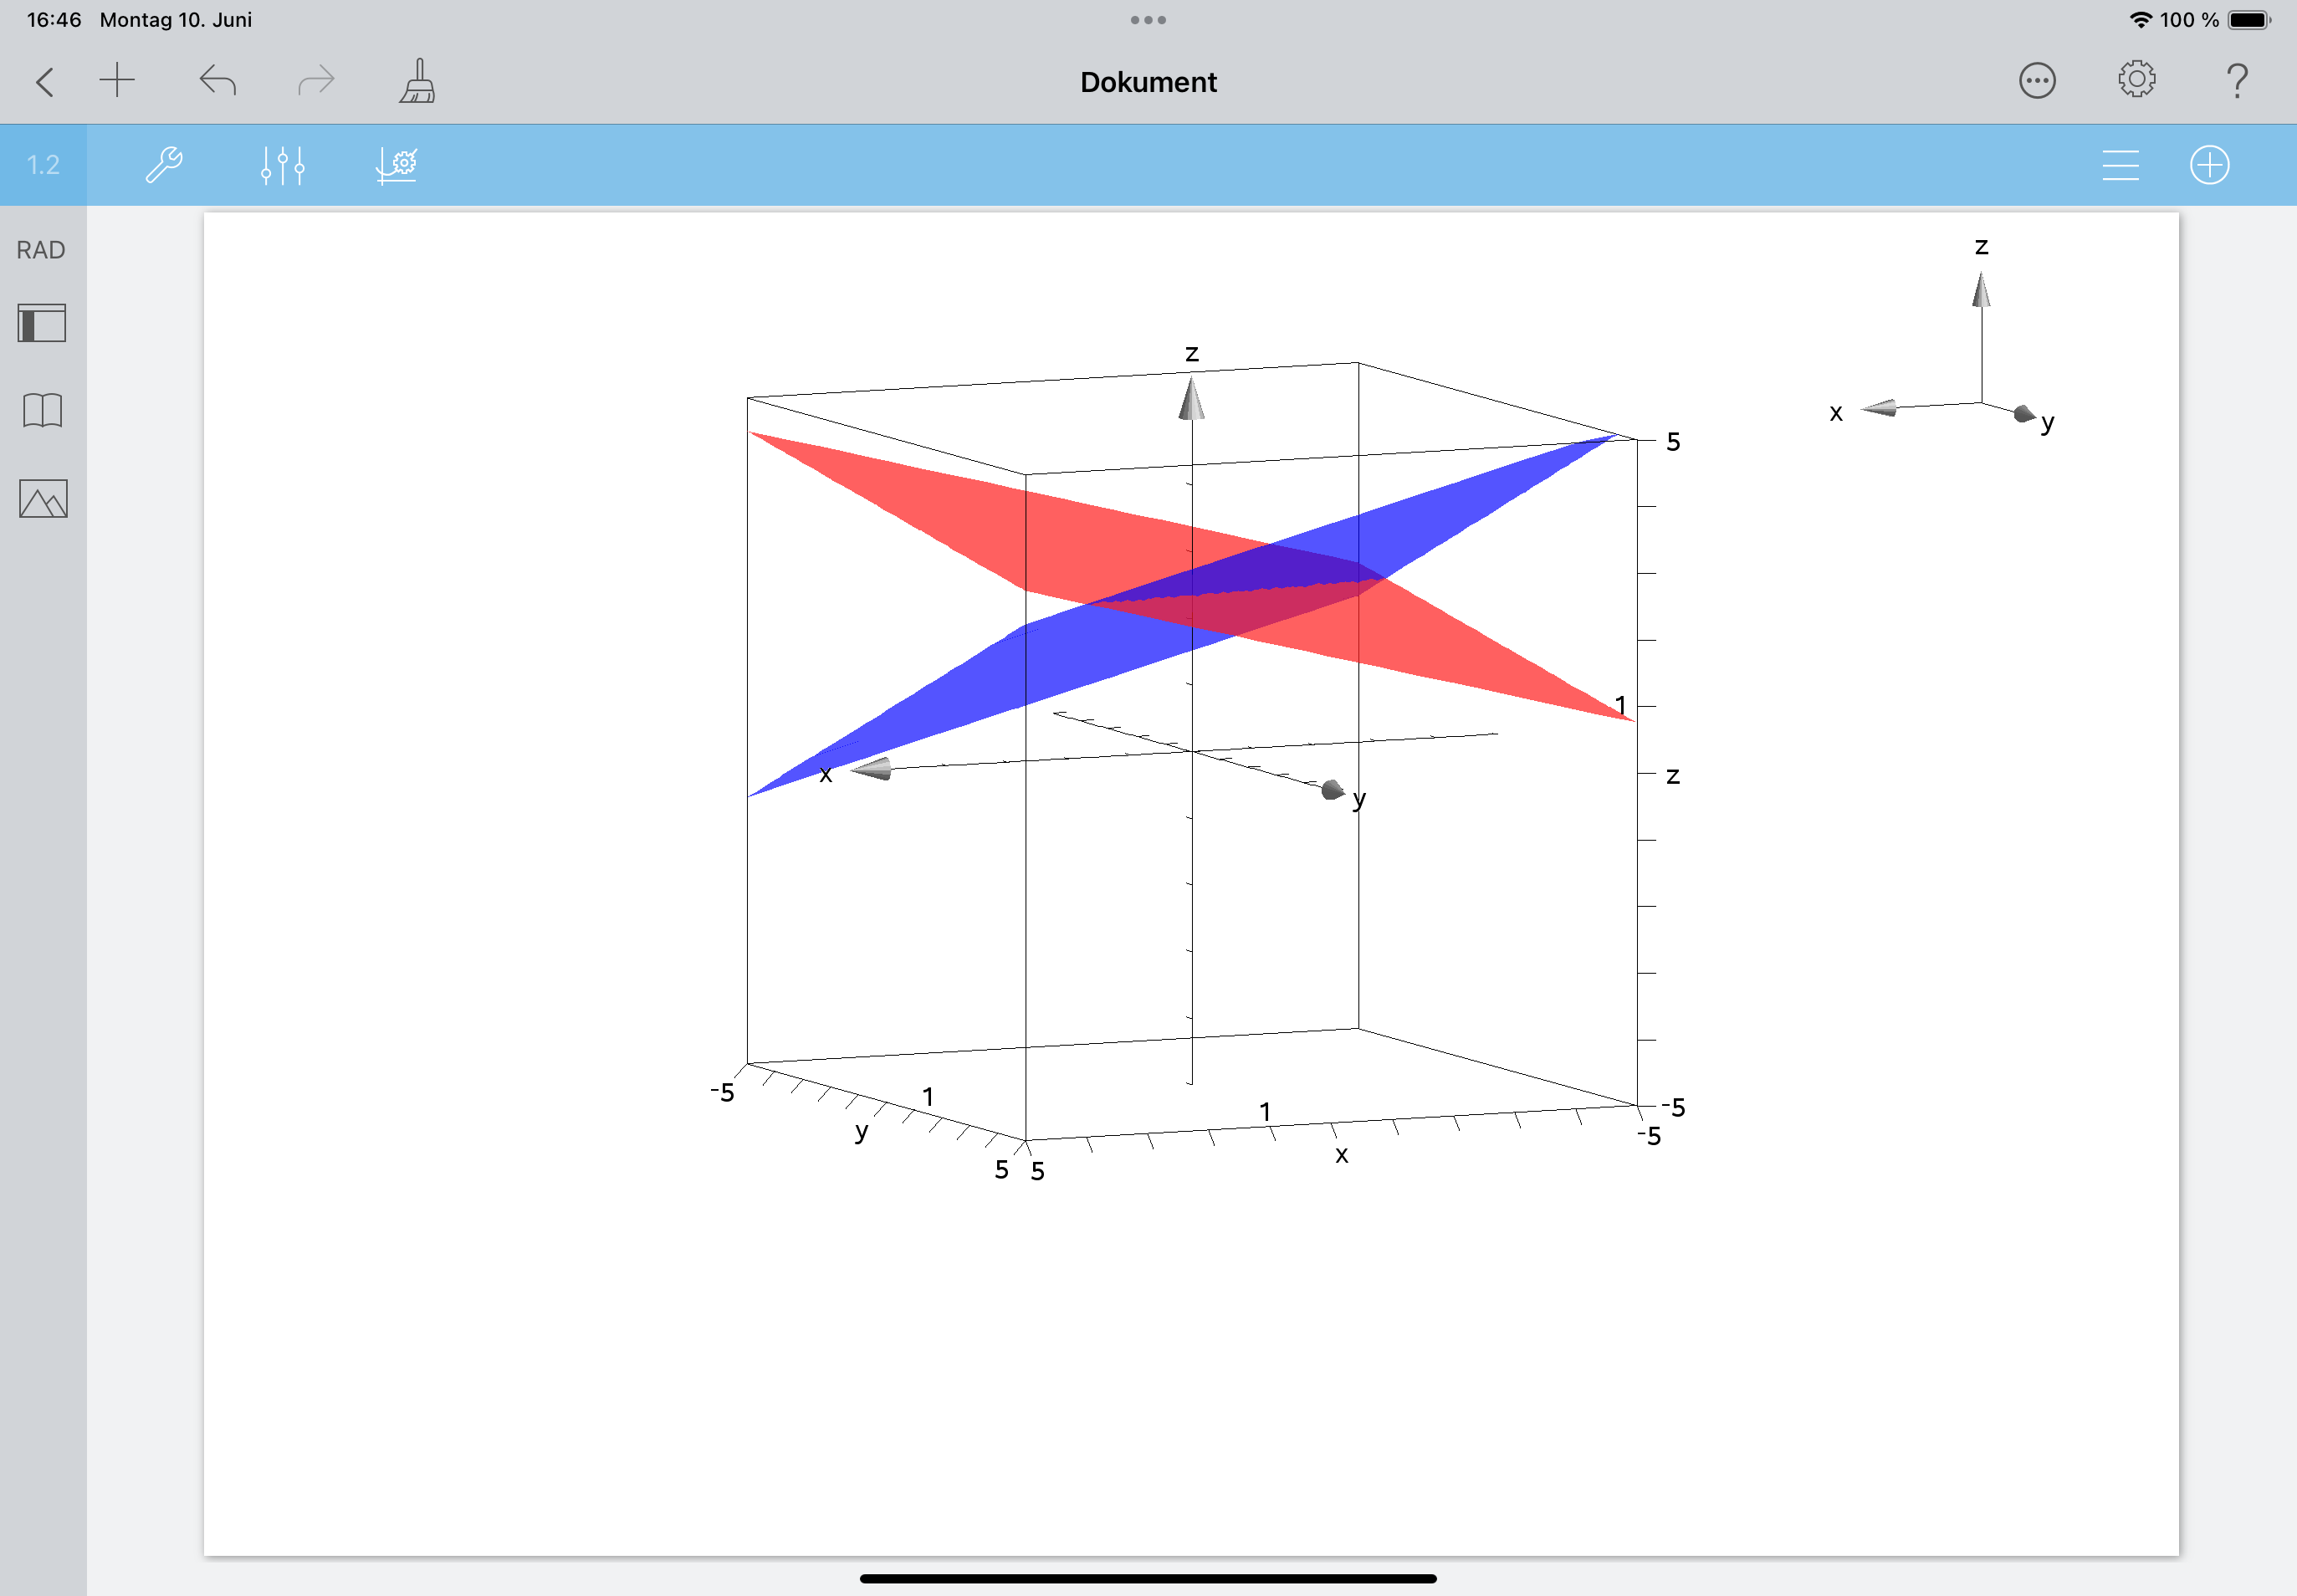
\includegraphics[width=\textwidth]{IMG_1449.png}
				\caption{Darstellung von zwei Ebenen}
				\label{fig:Darstellung-Zwei-Ebenen}
			\end{figure}
		\end{column}
	\end{columns}
\end{frame}

\subsection{Darstellung von Funktionen}

\begin{frame}
	\frametitle{Funktionen}

	\begin{columns}
		\begin{column}{0.5\textwidth}
			Man kann auch Funktionen darstellen, die zwei Parameter benutzen, wie die Darstellung einer harmonischen Welle.
		\end{column}

		\begin{column}{0.5\textwidth}
			\begin{figure}
				\centering
				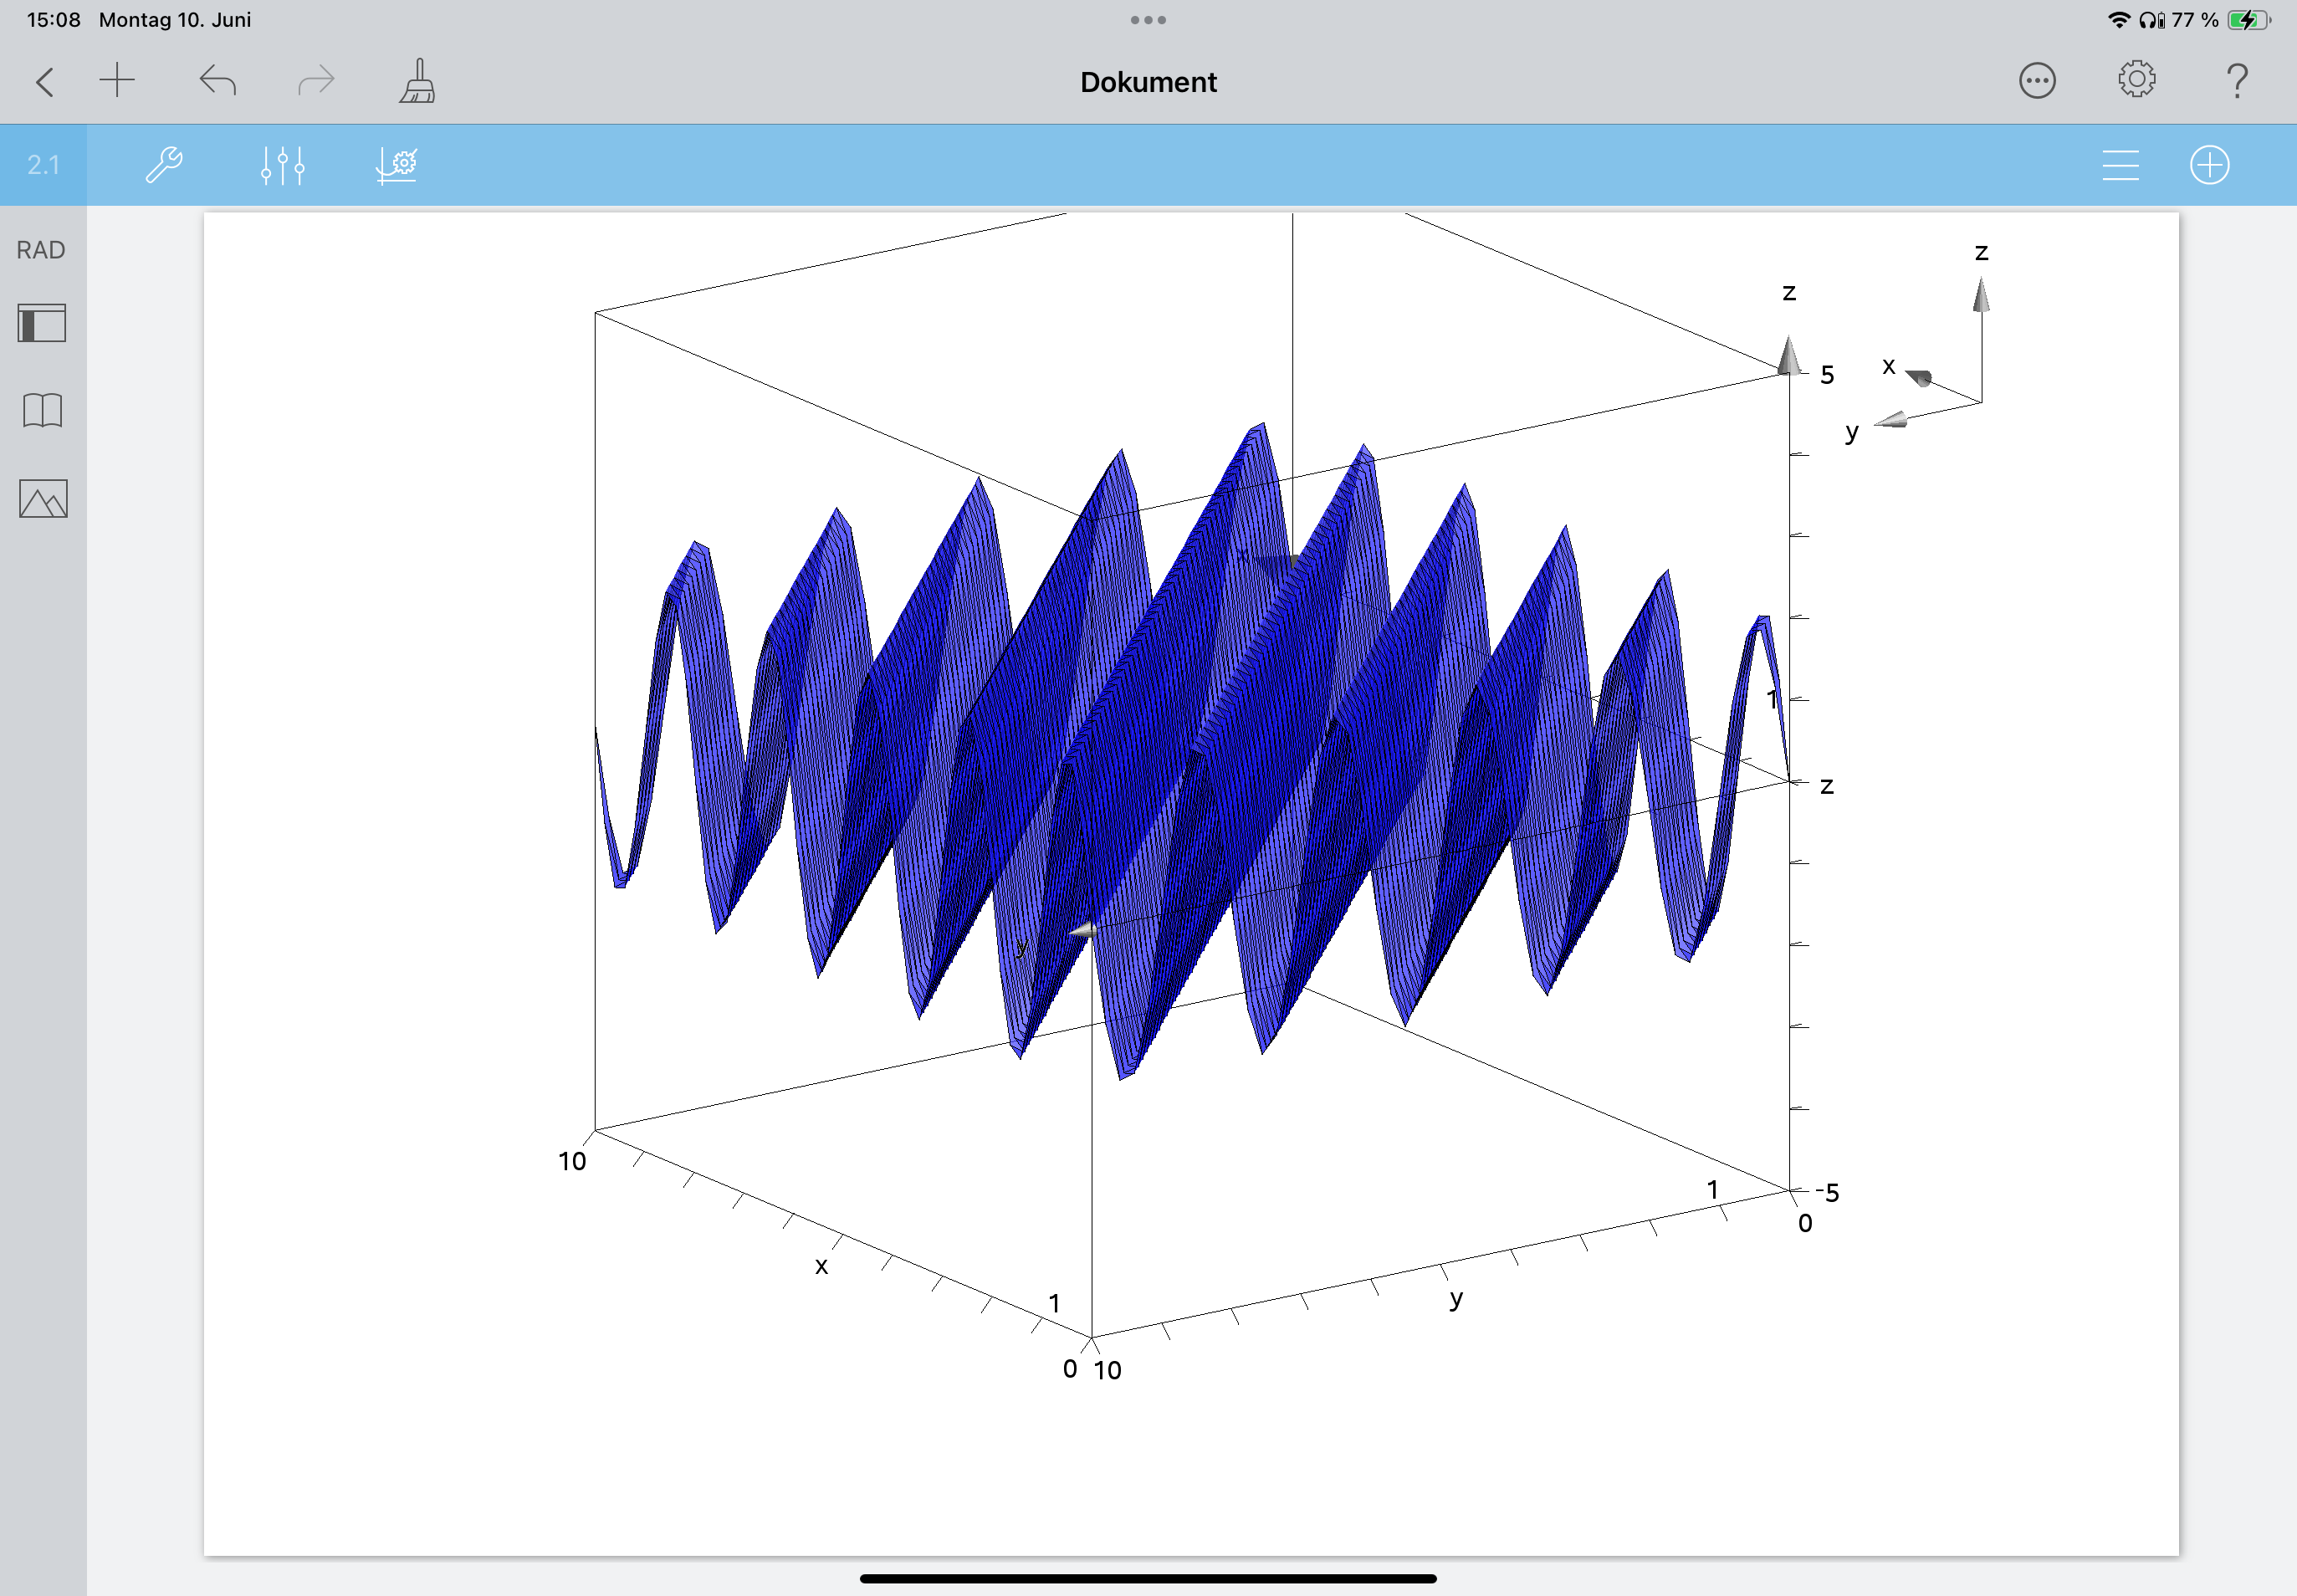
\includegraphics[width=\textwidth]{IMG_1448.png}
				\caption{Darstellung einer harmonischen Welle}
				\label{fig:Darstellung-Welle}
			\end{figure}
		\end{column}
	\end{columns}
\end{frame}

\begin{frame}
	\frametitle{Quellen}

	\begin{itemize}
		\item Abbildungen: \href{https://github.com/baumbus/ti}{GitHub} (10.06.2024 - 23:00)
		\item Quellcode für die Präsentation: \href{https://github.com/baumbus/ti}{GitHub} (10.06.2024 - 23:00)
	\end{itemize}
\end{frame}

\end{document}